\documentclass[11pt]{article}
\usepackage[scaled=0.92]{helvet}
\usepackage{geometry}
\geometry{letterpaper,tmargin=1in,bmargin=1in,lmargin=1in,rmargin=1in}
\usepackage[parfill]{parskip} % Activate to begin paragraphs with an empty line rather than an indent %\usepackage{graphicx}
\usepackage{amsmath,amssymb, mathrsfs, dsfont}
\usepackage{tabularx}
\usepackage[font=footnotesize,labelfont=bf]{caption}
\usepackage{graphicx}
\usepackage{xcolor}
%\usepackage[linkbordercolor ={1 1 1} ]{hyperref}
%\usepackage[sf]{titlesec}
\usepackage{natbib}
\usepackage{../../Tianpei_Report}

%\usepackage{appendix}
%\usepackage{algorithm}
%\usepackage{algorithmic}

%\renewcommand{\algorithmicrequire}{\textbf{Input:}}
%\renewcommand{\algorithmicensure}{\textbf{Output:}}



\begin{document}
\title{Lecture 2: Gauss Map and its Geometry}
\author{ Tianpei Xie}
\date{ Jun. 8th., 2015 }
\maketitle
\tableofcontents
\newpage
\section{The Definition of the Gauss Map and Its Fundamental Properties}
\subsection{Gauss Map}
\begin{itemize}
\item A \emph{\textbf{unit normal field}} in a neighborhood $U$ associate each point $p\in U\subset \cS$ the unit normal $N(p)$ at $p$ that is normal to the tangent space $T_{p}S$.

Given a parameterization $\mb{x}: U\subset \bR^{2} \rightarrow \cS$, the normal vector $N(p)$ at $p$ is given via
\begin{align*}
N(p) &= \frac{\mb{x}_{u} \wedge \mb{x}_{v}}{\abs{\mb{x}_{u} \wedge \mb{x}_{v}}}(p)
\end{align*}

If $V\subset \cS$ is an open subset in $\cS$ and $N: V\rightarrow \bR^{3}$ is a \emph{differentiable} map. It is called a \emph{\textbf{differentiable field of unit normal vectors}} on $V$.

\begin{figure}[thb]
\centering
\begin{minipage}{0.5\linewidth}
 \centerline{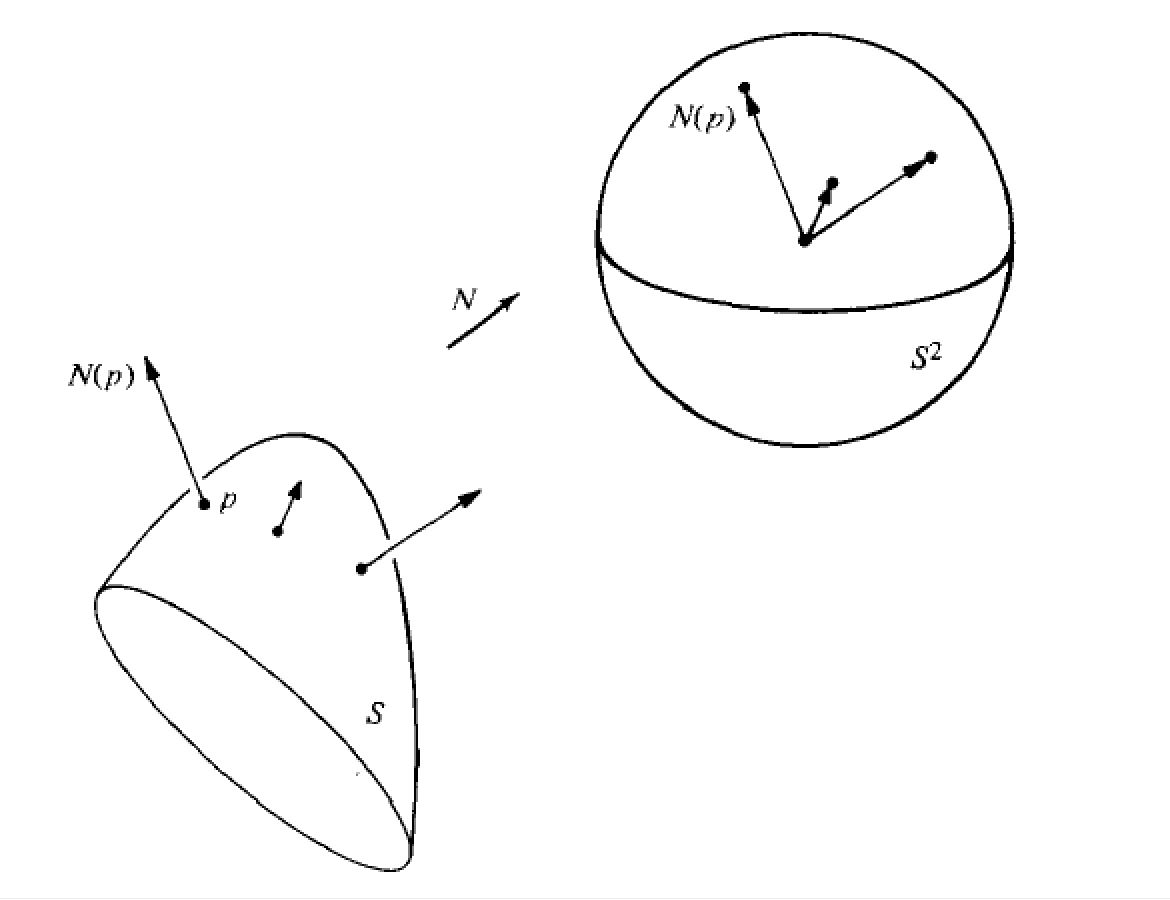
\includegraphics[scale = 0.5]{gauss_map.png}}
\end{minipage}
\caption{\scriptsize \textbf{The Gauss map from the surface to the unit sphere.}}
\end{figure}

\item The normal field may not be well-defined for the whole surface. A regular surface is \emph{\textbf{orientable}} if it admits a differentiable  field  of unit normal vectors defined on the whole surface. In terms of this, the choice of such a field $N$ is called an \emph{\textbf{orientation}} of $\cS$. Note that every surface is locally orientable, thus the orientation is a global property. 

 An orientation $N$ induces an orientation on $T_{p}S$, i.e. the basis $\set{v,w}$ is \emph{positive}, if $\inn{v\wedge w}{N}>0.$ The set of positive basis in $T_{p}S$ defines an orientation of the tangent space. 

 \item \begin{definition}
 Let $\cS\subset \bR^{3}$ be a surface with an orientation $N$. The map $N: \cS \rightarrow \bR^{3}$ takes its value in the unit sphere $\bS^{2}\equiv \set{(x,y,z)\in \bR^{3}|\;  x^{2}+ y^{2}+ z^{2} =1 }$.  The map $N: \cS \rightarrow \bS^{2}$ is called the \underline{\emph{\textbf{Gauss map}}} of $\cS$.
 \end{definition}
 
 \item $N$ is \textbf{differentiable} and $dN_{p}: T_{p}S \rightarrow T_{N(p)}\bS^{2}$ is a \emph{linear map}. Note that $T_{p}S$ and $T_{N(p)}\bS^{2}$ are parallel to each other, so $dN_{p}: T_{p}S \rightarrow T_{p}S$ is a \textbf{linear transformation} in $T_{p}S$. The differentiable of Gauss map is called the \emph{\textbf{shape operator}} \citep{o2006elementary}. 

\item In analogy as the curvature to the curve, $dN_{p}$ is the \emph{\textbf{rate of change}} at $p$ of a \emph{\textbf{unit normal vector field}} $N$  on a neighborhood of $p\in \cS$, which measures how rapidly the regular surface \emph{pull away from the tangent space} $T_{p}S$ at $p$.


\item For a parameterized curve $\alpha(t)$ on $\cS$ with $\alpha(0) = p$, we restrict the normal vector $N$ to the curve $\alpha(t)$ and $N_{p}(\alpha'(0)) \equiv N'(0)$ measures the rate of change of normal vectors, restricted on the curve $\alpha(t)$ at $t=0$. It thus measures how $N$ pull away from $N(p)$ in the neighborhood of $p$.  

In terms of this, \underline{\textbf{$dN_{p} $ to $\cS(u,v)$  is in analogy of $k(s)$ for curve $\alpha(s)$}}. As a linear mapping on the tangent space $T_{p}S$, $dN_{p}$ is an \emph{\textbf{extrinsic curvature}}. Its Jacobian determinant is the \underline{\emph{\textbf{Gaussian curvature}}}, an \emph{intrinsic curvature}, and its \textbf{trace} is the \emph{\textbf{mean curvature}}, an \emph{extrinsic curvature}. 

\begin{figure}[thb]
\centering
\begin{minipage}{0.5\linewidth}
 \centerline{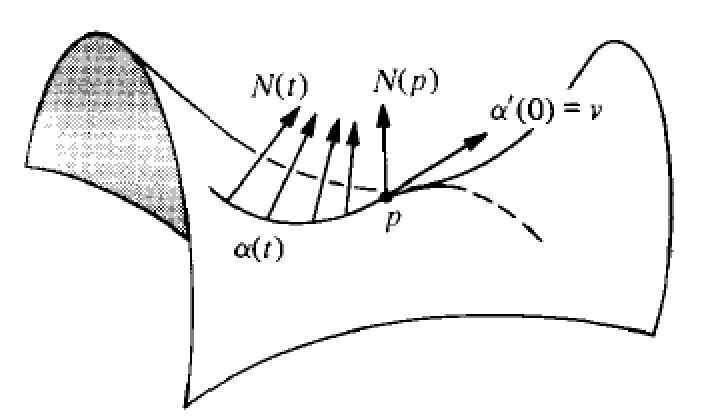
\includegraphics[scale = 0.55]{diff_gauss.png}}
\end{minipage}
\caption{\scriptsize
\textbf{The differential of Gauss map computed via restricting on the curve.}}
\end{figure}

\item (\textbf{Differential of normal vector field under basis})\\
For $p\in \cS$, $dN_{p}: T_{p}S \rightarrow T_{p}S$ is a linear transformation in $T_{p}S$. Let $\alpha(t) = \mb{x}(u(t), v(t))$ be a parameterized regular curve on surface $\cS$ with the tangent vector $\alpha'(t) = \mb{x}_{u}u'(t) + \mb{x}_{v}v'(t) $ under the basis $\set{\mb{x}_{u}, \mb{x}_{v}}$. Then 
\begin{align}
dN_{p}(\alpha'(t)) &= dN_{p}( \mb{x}_{u}u'(t) + \mb{x}_{v}v'(t) )\nonumber\\
&= \dfrac{d}{dt}N\paren{u(t), v(t)} = N_{u}u'(t) + N_{v}v'(t), \label{eqn: Gauss_map}
\end{align} where $N_{u} = dN_{p}( \mb{x}_{u})$ and  $N_{v} = dN_{p}( \mb{x}_{v})$. Note that $N_{u} \in T_{p}S$ and $N_{v} \in T_{p}S$, therefore
\begin{align}
N_{u}&= a_{11}\mb{x}_{u} + a_{21}\mb{x}_{v}\nonumber\\
N_{v}&= a_{12}\mb{x}_{u} + a_{22}\mb{x}_{v}. \label{eqn: Gauss_map_comp}
\end{align}
Note that $N(t) = N\circ \alpha(t)$ is a line on the unit sphere and $dN_{p}(\alpha') = N'(t)$ on the unit sphere. 

Under the basis $\set{\mb{x}_{u}, \mb{x}_{v}}$, 
\begin{align}
dN_{p}\,\paren{\begin{array}{c}
u'(t)  \\ 
v'(t) 
\end{array} } &= 
\brac{\begin{array}{cc}
a_{11} & a_{12} \\ 
a_{21} & a_{22}
\end{array} }\paren{\begin{array}{c}
u'(t)  \\ 
v'(t) 
\end{array} }  \label{eqn: Gauss_map_coord}
\end{align}
Note that if $\set{\mb{x}_{u}, \mb{x}_{v}}$ is not orthonormal, the above matrix $[a_{i,j}]$ is not necessary symmetric. The formula to compute these coefficients are called \emph{the Weingarten equations}. See \eqref{eqn: weingarten}. \\


\item \begin{proposition}\label{prop: Gauss_selfadj}
The differential $dN_{p}:  T_{p}S \rightarrow T_{p}S$ of the Gauss map is a self-adjoint linear map, i.e. $\inn{dN_{p}(\mb{w}_{1})}{\mb{w}_{2}} = \inn{\mb{w}_{1}}{dN_{p}(\mb{w}_{2})}  $ for $\set{\mb{w}_{1}, \mb{w}_{2}}$ any two vectors in $T_{p}S$. 
\end{proposition}
\begin{proof}
It suffice to show that $\inn{dN_{p}(\mb{w}_{1})}{\mb{w}_{2}} = \inn{\mb{w}_{1}}{dN_{p}(\mb{w}_{2})}  $ for $\set{\mb{w}_{1}, \mb{w}_{2}}$ the basis in $T_{p}S$. Let $\mb{x}(u,v)$ be a parameterization of the surface $\cS$ at $p$ and the $\set{\mb{x}_{u}, \mb{x}_{v}}$ be the basis for $T_{p}S$. If $\alpha(t) = \mb{x}(u(t), v(t))$ is a parameterized curve in $\cS$ with $\alpha(0) = p$, we have 
\begin{align*}
dN_{p}(\alpha'(0)) &= dN_{p}( \mb{x}_{u}u'(0) + \mb{x}_{v}v'(0) )\\
&= \rlat{\frac{d}{dt}N(u(t), v(t) )}{t=0}\\
&= dN_{u}u'(0) + dN_{v}v'(0)
\end{align*} with $dN_{u} = dN_{p}( \mb{x}_{u})$ and  $dN_{v} = dN_{p}( \mb{x}_{v})$.

To show the self-adjoint property, it suffice to show that $\inn{dN_{u}}{\mb{x}_{v}} = \inn{\mb{x}_{u}}{dN_{v}}$. To show this, we take derivative of $\inn{N}{\mb{x}_{u}} = 0$ and $\inn{N}{\mb{x}_{v}} = 0$ with respect to $v$ and $u$, respectively, and obtain
\begin{align*}
\inn{dN_{v}}{\mb{x}_{u}}  + \inn{N}{\mb{x}_{u,v}} = 0\\
\inn{dN_{u}}{\mb{x}_{v}}  + \inn{N}{\mb{x}_{v,u}} = 0
\end{align*}
Thus
\begin{align}
\inn{dN_{v}}{\mb{x}_{u}}  = -  \inn{N}{\mb{x}_{u,v}}  = \inn{dN_{u}}{\mb{x}_{v}}.  \label{eqn: the_2nd_fundamental_form_normal_curvature} 
\end{align}\QEDA
\end{proof}
\end{itemize}
\subsection{The Second Fundamental Form}
\begin{itemize}
\item The fact that $dN_p: T_{p}(\cS) \rightarrow T_p(\cS)$ is a self-adjoint linear map allows us to associate to $dN_p$ a quadratic form $Q$ in $T_p(\cS)$, given by $Q(v) = \inn{dN_{p}(v)}{v}, v \in T_{p}(\cS)$. 
\begin{definition}
 The \emph{quadratic form} $\Pi_{p}$ defined in \underline{$T_{p}\cS$} by $\Pi_{p}(\mb{v}) = -\inn{dN_{p}(\mb{v})}{\mb{v}}$ is called the \underline{\emph{\textbf{second fundamental form}}} of $\cS$ at $p$. 
\end{definition}

\item  Define the \emph{\textbf{normal curvature}} of a regular curve $\cC$ on a regular surface $\cS$ passing through a point $p\in \cC \subset \cS$. 
\begin{definition}
For $\cC \subset \cS$ as a regular curve passing through $p\in \cS$, let $k$ be the curvature of $\cC$ at $p$ and $\cos(\theta) = \inn{\mb{n}}{N}$, where $\mb{n}$ is the normal vector of the curve $\cC$ and $N$ is the normal vector of the surface $\cS$ at $p$. Define $k_{n} = k\cos(\theta)$ as the \underline{\emph{\textbf{normal component}}} of the \emph{\textbf{acceleration}} vector $\alpha''(s)= k\,\mb{n}$ along the \emph{direction} of \emph{normal vector} $N(p)$ to the \emph{tangent plane} of the surface. The quantity $k_{n}$ is referred as the \underline{\emph{\textbf{normal curvature}}} of a regular curve $\cC$ at a regular surface $\cS$. 
\end{definition}
\begin{figure}[thb]
\centering
\begin{minipage}{0.6\linewidth}
 \centerline{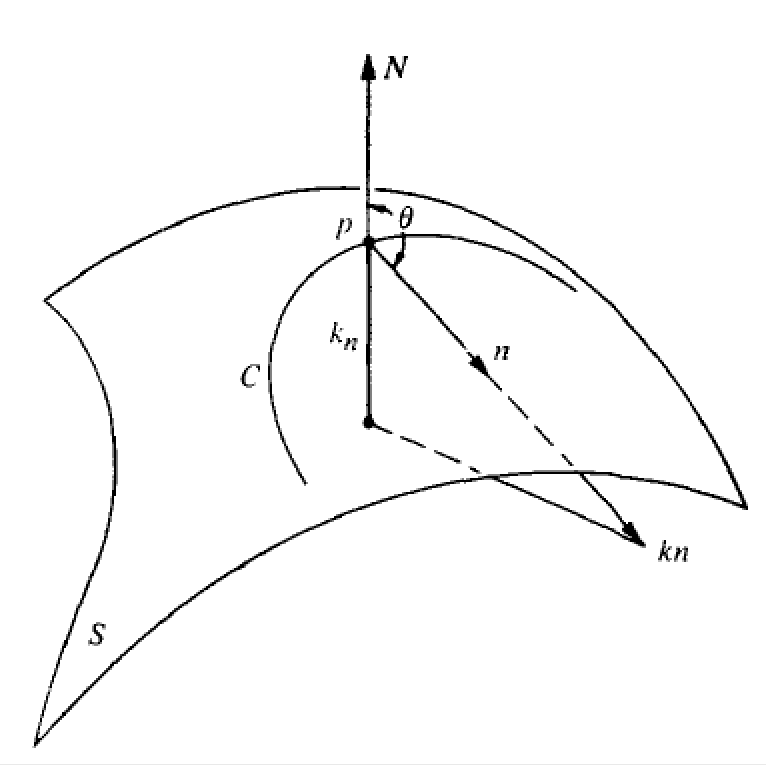
\includegraphics[scale = 0.43]{normal_curv.png}}
\end{minipage}
\caption{\scriptsize
\textbf{The normal curvature $k_{n}$ obtained by projection of $k\mb{n}$ the normal direction of curve $\cC$ to the direction of $N$, the normal direction to the tangent plane of $\cS$. }}
\end{figure}

%\item To give an interpretation of the second fundamental form $\Pi_{p}$, consider a regular curve $\cC \subset \cS$ parametrized by $\alpha(s)$, where $s$ is the arc length of $\cC$, and with $\alpha(0) = p$. If we denote by $N(s)$ the restriction of the normal vector $N$ to the curve $\alpha(s)$, we have $\inn{N(s)}{\alpha'(s)} = 0$. Hence,
%\begin{align}
%\inn{N(s)}{\alpha''(s)} &= - \inn{N'(s)}{\alpha'(s)}. \label{eqn: gauss_map_inn_product_accel}
%\end{align}
%Therefore,
%\begin{align}
%\Pi_{p}(\alpha'(0)) &= −\inn{dN_{p}(\alpha'(0))}{\alpha'(0)} \nonumber\\
%&= −\inn{N′(0)}{\alpha'(0)} = \inn{N(0)}{\alpha''(0)} \nonumber\\
%&= \inn{N}{k_n}(p) = k_n(p). \label{eqn: 2nd_fundamental_form_curvature}
%\end{align}
%In other words, the value of the \emph{\textbf{second fundamental form}} $\Pi_{p}$ for a unit vector $v \in T_p(\cS)$ is equal to the \emph{\textbf{normal curvature}} of a regular curve passing through $p$ and tangent to $v$. 

\item \begin{theorem}(\textbf{Meusnier}) \label{th: meusnier}\\
All curves lying on a surface $\cS$ and having at a given point $p\in \cS$ the same tangent line have at this point the same normal curvatures. 
\end{theorem}
\begin{figure}[thb]
\centering
\begin{minipage}{0.6\linewidth}
 \centerline{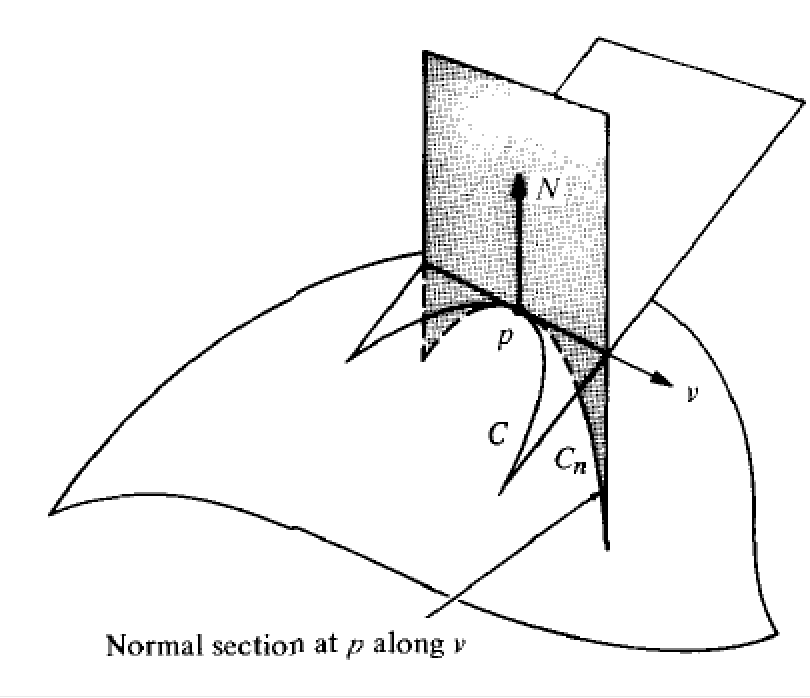
\includegraphics[scale = 0.43]{meusnier.png}}
\end{minipage}
\caption{\scriptsize
\textbf{The curve $\cC$ and $\cC_{n}$ have the same normal curvature. The dashed line $\cC_{n}$ is the normal section of $\cS$ at $p$ along the direction $\mb{v}$, which is the intersection between $\cS$ and the plane spanned by $N(p)$ and $\mb{v}$. By Meusnier's proposition, (the absolute value of) the normal curvature of the curve $\cC$ at $p$ (solid line) is equal to the  curvature of the normal section $\cC_{n}$ (dashed line) of $\cS$ at $p$ along $\alpha'(0)$. }}
\end{figure}
\begin{proof}
For the second fundamental form $\Pi_{p}$, consider a regular curve $\cC \subset \cS$ parameterized by $\alpha(s)$, where $s$ is the arc length, and $\alpha(0) = p$. If we denote by $N(s)$ the restriction of the normal vector $N$ to the curve $\alpha(s)$, we have $\inn{N(s)}{\alpha'(s)} = 0$. Hence 
\begin{align*}
\inn{N(s)}{\alpha''(s)} = - \inn{N'(s)}{\alpha'(s)}.
\end{align*}
Therefore
\begin{align*}
\Pi_{p}(\alpha'(0)) &= -\inn{dN_{p}(\alpha'(0))}{\alpha'(0)}\\
&= -\inn{N'(0)}{\alpha'(0)} = \inn{N(0)}{\alpha''(0)}\\
&= k\inn{N}{\mb{n}}(p) = k_{n}(p). 
\end{align*}

In other words, the value of \underline{\textbf{second fundamental form}} $\Pi_{p}(\mb{v})$ for unit vector $\mb{v}\in T_{p}S$ \textbf{is equal to} \underline{\textbf{the normal curvature}} of a regular curve passing through $p$ and tangent to $\mb{v}$. If $\mb{v}_{1} = \mb{v}_{2}$ for two curves $\cC_{1}$ and $\cC_{2}$, then $\Pi_{p}(\mb{v}_{1}) = k_{n1} = k_{n2} = \Pi_{p}(\mb{v}_{2})$. \QEDA
\end{proof}
The second fundamental form $\Pi_{p}(\mb{v})$ for any unit vector $\mb{v}\in T_{p}S$ is the \emph{normal curvature} of the $\cC$ passing through $p$ with $\alpha'(0) = \mb{v}$.

In fact, the \emph{\textbf{second fundamental form}} is the component of the \emph{second derivative} of parameterization $\mb{x}(u(t), v(t))$ \emph{\textbf{perpendicular}} to the \textbf{tangent plane} of $\cS$.

\item By theorem \ref{th: meusnier}, the normal curvature $k_{n}(p)$ is denoted as the \textbf{normal curvature} \emph{\textbf{along a given direction}} at $p$. 

The normal curvature measures the normal component of the curvature of an embedded curve $\cC$ on $\cS$ with respect to the tangent plane of the surface. It measures \emph{how rapidly the curve \textbf{pull away} from the entire \textbf{tangent space}}, as opposed to the original curvature that only measures the strength of the curve to deviate from a \emph{single tangent vector} along the curve in the tangent space. 

It is determined by the \textbf{angle} between \emph{the \textbf{osculating plane} of the curve} $\cC$ and \emph{the \textbf{tangent plane}} of the surface $\cS$ at the intersecting point $p\in \cS$. Note that $\mb{t}$ for the curve lies in both the osculating plane of the curve $\cC$ and the tangent plane of the surface $\cS$.


\item The intersection of $\cS$ with the plane containing the unit vector $\mb{v}\in T_{p}S$ and $N(p)$ is called the \emph{\textbf{normal section}} of $\cS$ at $p$ along $\mb{v}$. It is a plane curve with normal vector $\mb{n} = \pm N(p)$ or $0$. Its curvature is the absolute value of the normal curvature at $p$ along $\mb{v}$. 

Theorem \ref{th: meusnier} states that \emph{\textbf{the absolute value of the normal curvature}} at $p$ of a curve $\alpha(s)$ is equal to \emph{\textbf{the curvature of the normal section}} of $\cS$ at $p$ along $\alpha'(0)$.

\item If the surface is a plane, then all normal vectors are straight lines; hence, the  osculating plane of the curve $\cC$ and the tangent plane of the surface $\cS$ coincides and the normal curvature is zero. In terms of this, $dN_{p} \equiv 0$ for all $p$.

\item For given $dN_{p}$, there exists an orthonormal basis $\set{\mb{e}_{1}, \mb{e}_{2}}$ in $T_{p}S$ such that $dN_{p}(\mb{e}_{1}) = -k_{1}\mb{e}_{1}$ and  $dN_{p}(\mb{e}_{2}) = -k_{2}\mb{e}_{2}$, $(k_{1}\ge k_{2})$ i.e. $\set{\mb{e}_{1}, \mb{e}_{2}}$ are eigenvectors of $-dN_{p}$ associated with eigenvalues $(k_{1}, k_{2})$. We also see that 
$k_{1} = \max_{\norm{\mb{v}}{} = 1 }\Pi_{p}(\mb{v})$ and $k_{2} = \min_{\norm{\mb{v}}{} = 1 }\Pi_{p}(\mb{v})$.

\begin{definition}
The \emph{\textbf{maximum normal curvature}} $k_{1}$ and the \emph{\textbf{minimum normal curvature}} $k_{2}$ are called the \emph{\textbf{principal curvatures}} at $p$; the corresponding directions, that is, the direction given by the \textbf{eigenvectors} $\mb{e}_{1}$ and $\mb{e}_{2}$, are called \emph{\textbf{principal directions}} at $p$.
\end{definition}

\item For plane and sphere, all directions at all points are principal directions and the normal curvature are constant, i.e. the second fundamental form at every point, restricted to the unit vectors, is constant. For $\Pi_{p}(\mb{v}) = 0$ for all $p\in \cS$ and all $\norm{\mb{v}}{} = 1$, it is a plane, whereas  $\Pi_{p}(\mb{v}) = c$ for all $p\in \cS$ and all $\norm{\mb{v}}{} = 1$, it is a sphere with radius $1/c$. All directions are extremals for the normal curvature.

\item \begin{definition}
If a regular connected curve $\cC$ on $\cS$ is such that for every $p\in \cC$, the tangent line of $C$ is principal direction of surface at $p$, then $\cC$ is said to be a \emph{line of curvature of} $\cS$
\end{definition}

\item \begin{proposition} (\textbf{Olinde Rodrigues})\\
The necessary and sufficient condition for a curve $\alpha(t)$ to be a line of curvature is that
\begin{align*}
dN_{p}(\alpha'(t)) = N'(t) &= \lambda(t)\alpha'(t), 
\end{align*}where $N(t) = N\circ \alpha(t)$ and $
\lambda(t)$ is differentiable function of $t$ with $-\lambda(t)$ being the principal curvature of surface along $alpha'(t)$.
\end{proposition}

\item Given the principal curvature at $p$, one can compute the normal curvature $k_{n}$ at $p$ along any direction $\mb{v}\in T_{p}S$ with $\norm{\mb{v}}{} = 1$, as $\mb{v} = \mb{e}_{1}\cos(\theta) + \mb{e}_{2}\sin(\theta)$, where $\theta$ is the angle from $\mb{e}_{1}$ to $\mb{v}$. Hence
\begin{align}
k_{n} &= \Pi_{p}(\mb{v}) = -\inn{dN_{p}(\mb{v})}{\mb{v}}\nonumber\\
&= -\inn{dN_{p}( \mb{e}_{1}\cos(\theta) + \mb{e}_{2}\sin(\theta))}{ \mb{e}_{1}\cos(\theta) + \mb{e}_{2}\sin(\theta)}\nonumber\\
&= \inn{k_{1}\mb{e}_{1}\cos(\theta) + k_{2}\mb{e}_{2}\sin(\theta)}{\mb{e}_{1}\cos(\theta) + \mb{e}_{2}\sin(\theta)}\nonumber\\
&= k_{1}\cos(\theta)^{2} + k_{2}\sin(\theta)^{2}. \label{eqn: Euler_formula}
\end{align}
The above formula is called the \underline{\emph{\textbf{Euler formula}}}. This is the formula for the second fundamental form in the basis $\set{\mb{e}_{1}, \mb{e}_{2}}$ induced by the \textbf{principal directions}. 
\end{itemize}

\subsection{Gaussian Curvature and Shape of Surface}
\begin{itemize}
\item \begin{definition}
The \underline{\emph{\textbf{Gaussian curvature}}} $\mb{K}$ of $\cS$ at $p$ is defined as $\mb{K}\equiv \det\paren{dN_{p}}$ and the \emph{\textbf{mean curvature}} $\mb{H}$ is defined as $\mb{H}\equiv -\frac{1}{2}\text{trace}\paren{dN_{p}}$. 
\end{definition}
Note that $\mb{K} = k_{1}k_{2}$ for $k_{1}, k_{2}$ principal curvatures at $p$ and $\mb{H} = \frac{1}{2}\paren{k_{1}+ k_{2}}$.

\item A point $p$ of a surface $\cS$ is called
\begin{itemize}
\item \textbf{\emph{Elliptic}}, if $\mb{K}= \det\paren{dN_{p}} >0$.
All curves passing through an \emph{\textbf{elliptic}} point $p$ have their normal vector pointing towards the same side of the tangent plane. The principal curvatures are of the same sign and the Gaussian curvature is positive. 

\item \textbf{\emph{Hyperbolic}}, if $\mb{K}=\det\paren{dN_{p}} <0$. There are curves passing through an \emph{\textbf{hyperbolic}} point $p$ to have their normal vector pointing towards the any of the sides of the tangent plane. The principal curvatures are of the opposite sign and the Gaussian curvature is negative. 
\item \textbf{\emph{Parabolic}}, if  $\mb{K}=\det\paren{dN_{p}} =0$ but $dN_{p}\neq 0$. At \emph{\textbf{parabolic}} point $p$, the Gaussian curvature is zero, but one of the principal curvature is nonzero. The points of a cylinder, e.g., are parabolic points. 
\item \textbf{\emph{Planar}}, if $dN_{p} = 0$. At a \emph{\textbf{planar}} point, all principal curvatures are zero. The points in a plane satisfies this condition. An nontrival planer point, e.g. is the $(0,0,0)$ for the surface of revolution obtained by rotating the curve $z= y^{4}$ along the $z$-axis.  
\end{itemize}

\item \begin{definition}
If at $p$, the \emph{principal curvatures are the same} $k_{1} = k_{2}$, this point is called an \emph{\textbf{umbilical point}} of $\cS$; in particular, the planar points $k_{1}=k_{2} = 0$ are umbilical points. \citep{do1976differential}
\end{definition}

If all points of a connected surface $\cS$ are umbilical points, then $\cS$ is either a plane or a sphere.

\item  \begin{definition}
Let $p\in \cS$. An \emph{\textbf{asymptotic direction}} of $\cS$ at $p$ is a direction in $T_{p}S$ for which the normal curvature is zero. An \emph{\textbf{asymptotic curve}} of $\cS$ is a regular connected curve $\cC\subset \cS$ such that for each $p\in \cC$ the tangent line of $\cC$ at $p$ is an asymptotic direction. 
 \end{definition}
 
 It is clear that at elliptic point, there is no asymptotic directions. 
 
 \item For $p\in \cS$, the \emph{\textbf{Dupin indicatrix}} at $p$ is the set of vectors $\mb{w}$ of $T_{p}S$ such that $\Pi_{p}(\mb{w}) = \pm 1$.
 
 \item  (\textbf{Dupin indicatrix under basis})\\
Let $(\mb{e}_{1}, \mb{e}_{2})$ be the basis of $T_{p}S$ as the principal directions of $dN_{p}$. Then via a polar coordinate $\mb{w} = \rho\,\mb{v}$ and $\mb{v} = \xi\mb{e}_{1}+ \eta\mb{e}_{2}$. By Euler's formula, the Dupin indicatrix satisfies the following equation
 \begin{align*}
 \pm 1 = \Pi_{p}(\mb{w}) &= \rho^{2}\,\Pi_{p}(\mb{v})\\
 &= k_{1}\rho^{2}\cos^{2}(\theta) + k_{2}\rho^{2}\sin^{2}(\theta) \\
 &= k_{1}\xi^{2} + k_{2}\eta^{2}.
 \end{align*}
Thus the set of coordinates $(\xi, \eta)$ satisfies the Dupin indicatrix is the a union of conics in $T_{p}S$. The normal curvature along the direction $\mb{w}$ is $k_{n}(\mb{v}) = \pm \frac{1}{\rho^{2}}$.

It is clear that 
\begin{itemize}
\item For an \emph{\textbf{elliptic point}}, the Dupin indicatrix is an \emph{ellipse}, i.e. $k_{1}\xi^{2} + k_{2}\eta^{2} = 1$. 
\item For an \emph{\textbf{hyperbolic point}}, the Dupin indicatrix is made of \emph{two hyperbolas with a common pair of asymptotic lines}, i.e. i.e. $k_{1}\xi^{2} + k_{2}\eta^{2} = -1$. Along the direction of asymptotes, the normal curvature is zero; they are therefore the asymptotic directions. A hyperbolic point has exactly two asymptotic directions.  
\item For a \emph{\textbf{parabolic point}}, the Dupin indicatrix degenerates into a pair of \emph{parallel lines} as one of the principal curvature is zero. The common direction of these lines is the only asymptotic directions at the given point. 
\end{itemize}

\begin{figure}[thb]
\centering
\begin{minipage}{0.8\linewidth}
 \centerline{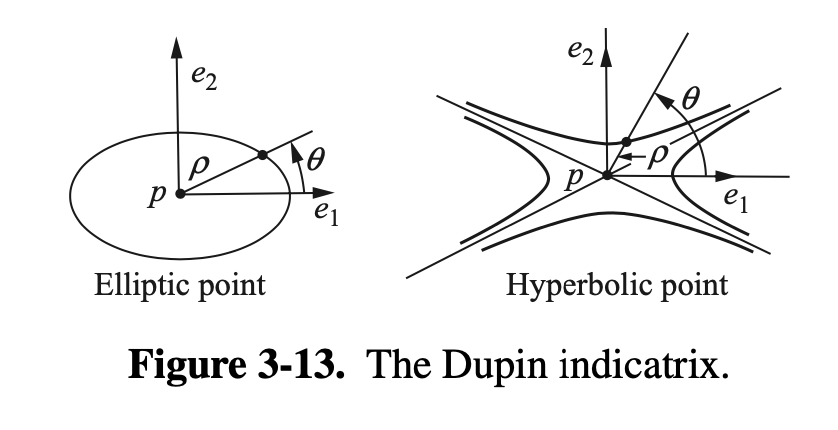
\includegraphics[scale = 0.43]{dubinmatrix.png}}
\end{minipage}
\caption{\scriptsize
\textbf{The dupin indicatrix for elliptic and hyperbolic point.}}
\label{fig: dubinmatrix}
\end{figure}



 
\item \begin{definition}
At a point $p\in \cS$, two nonzero vectors $\mb{w}_{1}$ and $\mb{w}_{2}$ in $T_{p}S$ are \emph{\textbf{conjugate}}, if $\inn{dN_{p}(\mb{w}_{1})}{\mb{w}_{2}} = \inn{\mb{w}_{1}}{dN_{p(\mb{w}_{2})}} = 0$. Two directions $\mb{r}_{1}$ and $\mb{r}_{2}$ at $p$ are \emph{\textbf{conjugate}} if a pair of nonzero vectors  $\mb{w}_{1}$ and $\mb{w}_{2}$ parallel to $\mb{r}_{1}$ and $\mb{r}_{2}$, respectively, are \emph{conjugate}. 
\end{definition}

Note that all principal directions are conjugate. The asymptotic directions are conjugate to itself. At a nonplanar umbilic, every pair of orthogonal directions are conjugate directions and at a planar umbilic, any two directions are conjugate. 

\item
For $p\in \cS$, and the basis $\set{\mb{e}_{1}, \mb{e}_{2}}$ are basis of $T_{p}S$ given by the principal directions. Let $\theta$ and $\varphi$ be the angles that a pair of directions $\mb{r}_{1}$ and $\mb{r}_{2}$ make with $\mb{e}_{1}$. Then two directions $\mb{r}_{1}$ and $\mb{r}_{2}$ are conjugate iff 
\begin{align*}
k_{1}\cos(\theta)\cos(\varphi) &= - k_{2}\sin(\theta)\sin(\varphi)
\end{align*}

\item For \textbf{elliptic} (or \textbf{hyperbolic}) points, the conjugate direction can be constructed using \emph{Dupin indicatrix} at $p$. 
\begin{enumerate}
\item For given direction $\mb{r}_{1}$, we construct a straight line with $\mb{r}_{1}$ direction going through the origin of $T_{p}S$.
\item Then we find the intersection point of $\mb{r}_{1}$ with the Dupin indicatrix $\set{(\xi, \eta)\;| \;\;k_{1}\xi^{2} + k_{2}\eta^{2} = 1}$ as $q_{1}, q_{2}$. 
\item The tangent line of the Dupin indicatrix at these two points are parallel lines with common direction $\mb{r}_{2}$ that is \emph{conjugate} to $\mb{r}_{1}$.
\end{enumerate}
\end{itemize}

\section{The Gauss Map in Local Coordinates}
\subsection{Calculations}
\begin{itemize}
\item (\emph{\textbf{The Second Fundamental Form under basis}})\\
Given the basis $\set{\mb{x}_{u}, \mb{x}_{v}}$ in $T_{p}S$ at $p\in \cS$, and let $\alpha(t) = \mb{x}(u(t), v(t))$ be a parameterized regular curve on surface $\cS$ with the tangent vector $\alpha'(t) = \mb{x}_{u}u'(t) + \mb{x}_{v}v'(t) $ under the basis $\set{\mb{x}_{u}, \mb{x}_{v}}$ and $p=\alpha(0)= \mb{x}(u(0), v(0))$. The second fundamental form is computed as
\begin{align}
\Pi_{p}(\alpha') &=  -\inn{dN_{p}(\alpha')}{\alpha'}\nonumber\\
&= -\inn{N_{u}u'(t) + N_{v}v'(t)}{ \mb{x}_{u}u'(t) + \mb{x}_{v}v'(t)}\nonumber\\
&= e\paren{u'(t)}^{2} + 2f\paren{u'(t)v'(t)} + g\paren{v'(t)}^{2} \label{eqn: second_fund_form_2}
\end{align}
where the coefficient for the second fundamental form is given as 
\begin{align}
e(u(0), v(0))&= - \inn{N_{u}}{\mb{x}_{u}} = \inn{N}{\mb{x}_{uu}} \nonumber\\
f(u(0), v(0))&= - \inn{N_{u}}{\mb{x}_{v}} =  \inn{N}{\mb{x}_{vu}} =  \inn{N}{\mb{x}_{uv}} =  -\inn{N_{v}}{\mb{x}_{u}}\nonumber\\
g(u(0), v(0))&=   - \inn{N_{v}}{\mb{x}_{v}} = \inn{N}{\mb{x}_{vv}}  \label{eqn: second_fund_coeff}
\end{align}
and the last equality in each row comes by differentiating both equations $\inn{N}{\mb{x}_{u}} = 0$ and $\inn{N}{\mb{x}_{v}} = 0$ with respect to either $u$ or $v$, respectively. 

We can compute these coefficients from $\set{\mb{x}_{uu},\mb{x}_{uv}, \mb{x}_{vv}, N }$. In specific, by using the formula in \eqref{eqn: second_fund_coeff}
\begin{align}
e &= \inn{N}{\mb{x}_{uu}} = \inn{\frac{\mb{x}_{u} \wedge \mb{x}_{v}}{\abs{\mb{x}_{u} \wedge \mb{x}_{v}}}}{\mb{x}_{uu}}= \frac{\det\paren{ \mb{x}_{u} , \mb{x}_{v}, \mb{x}_{uu}  }}{EG- F^{2}} \nonumber\\
f &= \inn{N}{\mb{x}_{uv}} = \inn{\frac{\mb{x}_{u} \wedge \mb{x}_{v}}{\abs{\mb{x}_{u} \wedge \mb{x}_{v}}}}{\mb{x}_{uv}}= \frac{\det\paren{ \mb{x}_{u} , \mb{x}_{v}, \mb{x}_{uv}  }}{EG- F^{2}} \nonumber\\
g &= \inn{N}{\mb{x}_{uu}} = \inn{\frac{\mb{x}_{u} \wedge \mb{x}_{v}}{\abs{\mb{x}_{u} \wedge \mb{x}_{v}}}}{\mb{x}_{vv}}= \frac{\det\paren{ \mb{x}_{u} , \mb{x}_{v}, \mb{x}_{vv}  }}{EG- F^{2}} \label{eqn: second_fund_coeff_2}
\end{align}



By the matrix $[a_{i,j}]$ in \eqref{eqn: Gauss_map_coord}, and the coefficient for the first fundamental form, 
\begin{align}
-f &=  \inn{N_{u}}{\mb{x}_{v}} = \inn{a_{11}\mb{x}_{u} + a_{21}\mb{x}_{v}}{\mb{x}_{v}} = a_{11}F + a_{21}G, \nonumber\\
-f &=  \inn{N_{v}}{\mb{x}_{u}} = \inn{a_{12}\mb{x}_{u} + a_{22}\mb{x}_{v}}{\mb{x}_{u}} = a_{12}E + a_{22}F, \nonumber\\
-e &= \inn{N_{u}}{\mb{x}_{u}}  = \inn{a_{11}\mb{x}_{u} + a_{21}\mb{x}_{v}}{\mb{x}_{u}} = a_{11}E + a_{21}F, \nonumber\\
-g &= \inn{N_{v}}{\mb{x}_{v}}  = \inn{a_{12}\mb{x}_{u} + a_{22}\mb{x}_{v}}{\mb{x}_{v}} = a_{12}F + a_{22}G. \label{eqn: second_fund_coeff_3} 
\end{align}
From \eqref{eqn: second_fund_coeff_3}, in matrix form, we have
\begin{align}
-\brac{\begin{array}{cc}
e & f \\ 
f & g
\end{array} }
&= 
\brac{\begin{array}{cc}
a_{11} & a_{21} \\ 
a_{12} & a_{22}
\end{array} }
\brac{\begin{array}{cc}
E & F \\ 
F & G
\end{array} }
\end{align}
One can compute the coefficients $[a_{i,j}]$ as
\begin{align*}
\brac{\begin{array}{cc}
a_{11} & a_{21} \\ 
a_{12} & a_{22}
\end{array} }
&= -\brac{\begin{array}{cc}
e & f \\ 
f & g
\end{array} }
\brac{\begin{array}{cc}
E & F \\ 
F & G
\end{array} }^{-1}
\end{align*} or
\begin{align}
a_{11} &= \frac{fF- eG}{EG- F^{2}} \nonumber\\
a_{12} &= \frac{gF- fG}{EG- F^{2}} \nonumber\\
a_{21} &= \frac{eF- fE}{EG- F^{2}} \nonumber\\
a_{22} &= \frac{fF- gE}{EG- F^{2}} \label{eqn: weingarten}
\end{align}
which is called the \emph{\textbf{equations of Weingarten}} \citep{do1976differential}. 

\item Given the coefficients for the Second Fundamental Form $(e,f,g)$ and those for the First Fundamental Form $(E,F,G)$, the \emph{\textbf{Gaussian curvature}} can be computed as 
\begin{align}
\mb{K} &= \det\brac{a_{i,j}} = \frac{eg- f^{2}}{EG- F^{2}} \label{eqn: Gaussian_curvature}
\end{align}



\item  The \emph{\textbf{principal curvature}} $(k_{1}, k_{2})$ is the \textbf{eigenvalue} of $-dN_{p}$, which is the solution of equations
\begin{align*}
\det\brac{\begin{array}{cc}
a_{11}+ k & a_{12} \\ 
a_{21} & a_{22}+k
\end{array} } = 0
\end{align*} or
\begin{align*}
k^{2}+ k(a_{11}+ a_{22}) + a_{11}a_{22} - a_{12}a_{21} = 0
\end{align*}
\begin{align}
k &= \mb{H} \pm \sqrt{\mb{H}^{2}- \mb{K}}  \label{eqn: principal_curv_coord}
\end{align}
where the \emph{\textbf{mean curvature}} is 
\begin{align}
\mb{H} &= -\frac{1}{2}(a_{11}+ a_{22}) = \frac{1}{2}\frac{eG - 2fF + gE}{EG-F^{2}}
\end{align}


\item \begin{proposition}
Let $p \in \cS$ be an \textbf{elliptic point} of a surface $\cS$. Then there exists a neighborhood $V$ of $p$ in $\cS$ such that all points in $V$ belong to the \textbf{same side of the tangent plane} $T_{p}(\cS)$. Let $p \in \cS$ be a \textbf{hyperbolic point}. Then in each neighborhood of $p$ there exist points of $\cS$ in \textbf{both sides} of $T_{p}(\cS)$.
\end{proposition}



\item (\emph{\textbf{Asymptotic directions under basis}})\\
A connected regular curve $\cC$ in the coordinate neighborhood of $\mb{x}$ as $\alpha(t) = \mb{x}(u(t), v(t)), t\in I$ is an \emph{asymptotic curve} iff $\Pi(\alpha'(t)) = 0$ for all $t\in I$. Then it follows that
\begin{align}
e(u')^{2} + 2f(u'v') + g(v')^{2} = 0,\quad t\in I \label{eqn: diff_eqn_asym_curve}
\end{align}
is called the \emph{\textbf{differential equation for the asymptotic curves}}. 

A direct conclusion from \eqref{eqn: diff_eqn_asym_curve} is that for the \emph{hyperbolic point} $p\in \cC\subset \cS$, a necessary and sufficient condition for a parameterization $\mb{x}$ in its neighborhood to be such that the coordinate curves of the parameterization are asymptotic curves is that $e= g= 0$.

\item (\emph{\textbf{Principal directions under basis}})\\
A connected regular curve $\cC$ the coordinate neighborhood of $\mb{x}$ as $\alpha(t) = \mb{x}(u(t), v(t)), t\in I$ is a \emph{line of curvature} iff for any paramterization $\mb{x}$, we have 
\begin{align*}
dN(\alpha'(t)) &= \lambda(t)\alpha'(t)
\end{align*}
Thus
\begin{align*}
\brac{\begin{array}{cc}
a_{11} & a_{21} \\ 
a_{12} & a_{22}
\end{array} }\brac{\begin{array}{c}
u' \\ 
v'
\end{array} } &= \lambda\,\brac{\begin{array}{c}
u' \\ 
v'
\end{array} }
\end{align*}
Thus by \eqref{eqn: weingarten} and eliminating $\lambda$, we have
\begin{align}
&(fE- eF)(u')^{2} + (gE-eG)(u'v')+ (gF-fG)(v')^{2} = 0\nonumber\\[5pt]
\text{or }& 
\det\abs{\begin{array}{ccc}
(v')^{2} & -(u'v') & (u')^{2}  \\ 
E & F & G \\ 
e & f & g
\end{array} } = 0, \label{eqn: diff_eqn_line_curvature}
\end{align} which is called the \emph{\textbf{differential equation for the lines of curvature}}.

Note that the principal directions are orthogonal to each other $(u'v' =0)$, it concludes from \eqref{eqn: diff_eqn_line_curvature} that a necessary and sufficient condition for the coordinate curves of a parameterization to be lines of curvature in a neighborhood of a nonumbilical point is that $F=f = 0$. 
\end{itemize}


\subsection{Geometrical interpretation of the Gaussian curvature}
\begin{itemize}
\item \begin{proposition}
Let $p$ be a point of a surface $\cS$ such that the Gaussian curvature $\mb{K}(p) \neq 0$, and let $V$ be a \textbf{connected} neighborhood of $p$ where $\mb{K}$ does not change sign. Then
\begin{align*}
\mb{K}(p) &= \lim_{A\rightarrow 0}\frac{A'}{A}, 
\end{align*}
where $A$ is the area of a region $B \subset V$ containing $p$, $A'$ is the area of the image of $B$ by the \textbf{Gauss map} $N: \cS \rightarrow \bS^2$, and the limit is taken through a sequence of regions $(B_n)$ that converges to $p$, in the sense that any sphere around $p$ contains \textbf{all} $B_n$, for $n$ sufficiently large.
\end{proposition}

\item \begin{definition}
Let $\cS$ and $\cS'$ be two \emph{oriented regular surfaces}. Let $\varphi: \cS \rightarrow \cS '$ be a differentiable map and assume that for some $p \in \cS$, $d\varphi_{p}$ is \emph{nonsingular}. 

We say that $\varphi$ is \emph{\textbf{orientation-preserving}} at $p$ if given a positive basis $\set{\mb{w}_1 , \mb{w}_2}$ in $T_{p}(\cS)$, then $\set{d\varphi_{p}(\mb{w}_1), d\varphi_{p}(\mb{w}_2)}$ is a \emph{\textbf{positive basis}} in $T_{\varphi(p)}(\cS')$. If $\set{d\varphi_{p}(\mb{w}_1), d\varphi_{p}(\mb{w}_2)}$ is not a positive basis, we say that $\varphi$ is \emph{\textbf{orientation-reversing}} at $p$.
\end{definition}

\begin{figure}[tb]
\centering
\begin{minipage}{0.5\linewidth}
 \centerline{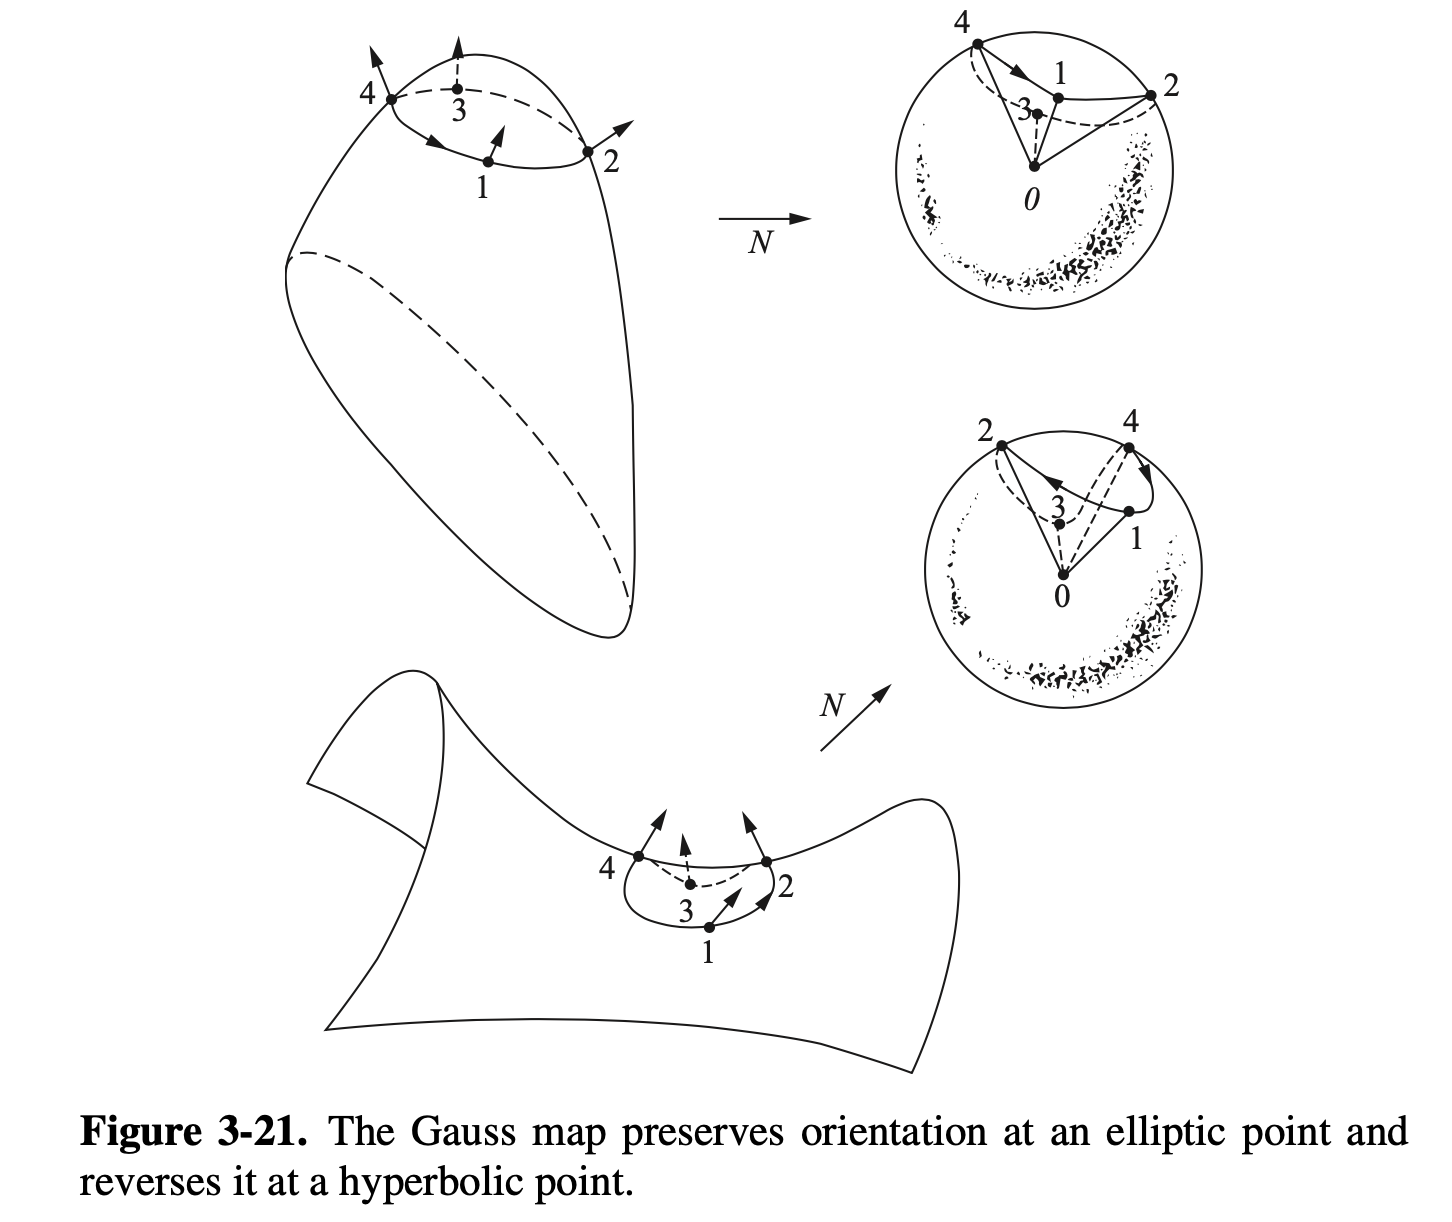
\includegraphics[scale = 0.55]{guassian_curve_via_gaussian_map.png}}
\end{minipage}
\caption{\scriptsize
\textbf{Gauss map is orientation-preserving if Gaussian curvature is positive, and is orientation-reserving if Gaussian curvature is negative}}
\label{fig: guassian_curve_via_gaussian_map}
\end{figure}

\item We now observe that both $\cS$ and the unit sphere $\bS^2$ are embedded in $\bR^3$. Thus, an \emph{orientation} $N$ on $\cS$ induces an orientation $N$ in $\bS^2$. Let $p \in \cS$ be such that $dN_{p}$ is \emph{nonsingular}. 

Since for a basis $\set{\mb{w}_1 , \mb{w}_2}$ in $T_{p}(\cS)$
\begin{align*}
dN_{p}(\mb{w}_1) \wedge dN_{p}(\mb{w}_2) &= \det(dN_{p})(\mb{w}_1 \wedge \mb{w}_2) = \mb{K}\,\mb{w}_1 \wedge \mb{w}_2,
\end{align*} the \emph{\textbf{Gauss map}} $N$ will be \emph{\textbf{orientation-preserving}} at $p \in \cS$ if $\mb{K}(p) > 0$ and \emph{\textbf{orientation-reversing}} at $p \in \cS$ if $\mb{K}(p) < 0$. 

Intuitively, this means the following (Figure \ref{fig: guassian_curve_via_gaussian_map}): An orientation of $T_{p}(\cS)$ \emph{induces an orientation} of small closed curves in $\cS$ around $p$; the image by $N$ of these curves will have the \emph{same} or the \emph{opposite} \emph{orientation} to the initial one, depending on whether $p$ is an \emph{\textbf{elliptic}} or \emph{\textbf{hyperbolic point}}, respectively.

To take this fact into account we shall make the convention that the area of the image by $N$ of a region contained in a connected neighborhood $V \subset S$ where  $\mb{K}(p) \neq 0$ is positive if $\mb{K} > 0$ and negative if $\mb{K} < 0$ (since $V$ is connected, $\mb{K}$ does not change sign in $V$).
\end{itemize}


\section{Summary of shape operator $dN_{p}$}
\begin{enumerate}
\item The shape operator $dN_{p}: T_{p}S \rightarrow T_{p}S$ is a linear operator on the tangent space $T_{p}S$. It defines many intrinsic and extrinsic property of the surface. It is a self-adjoint operator. 

\item $dN_{p}(\mb{v})$ is the rate of change of the unit normal field $\mb{N}(p)$ along direction $\mb{v}$. As the normal field on the unit sphere, its rate of change will always be tangent to the surface, thus $dN_{p}(\mb{v}) \in T_{p}S$.

\item The determinant $\det{dN_{p}}$  is the Gaussian curvature $\mb{K}$, which is an intrinsic curvature of the surface, i.e. it is invariant under isometries. 

\item The trace $-\text{tr}\paren{dN_{p}}$ is called the mean curvature $\mb{H}$, which is an extrinsic curvature of the surface. 

\item The quadratic form of $\Pi_{p}(\mb{v}) = \inn{-dN_{p}(\mb{v})}{\mb{v}},$ for all $\mb{v}\in T_{p}S$ is the second fundamental form. It is the normal curvature of the surface along unit length direction $\mb{v}/\abs{\mb{v}}$ or the curvature of the normal section of the surface along direction $\mb{v}$. 

The second fundamental form is associated with the projection of the second-order derivatives of the parameterization along the normal direction of the surface. 

The second fundamental form is invariant under reparameterization and isometries. 
 
\item The eigenvalues and eigenvectors of $dN_{p}$ is called the principal curvature and the principal directions. It is given as the set of recursively maximum normal curvatures along a set of orthonormal directions.  

\item A point $p$ of a surface $\cS$ is called
\begin{itemize}
\item Elliptic, if $\mb{K}= \det\paren{dN_{p}} >0$; \\
All curves passing through an \emph{elliptic} point $p$ have their normal vector pointing towards the same side of the tangent plane. The principal curvatures are of the same sign and the Gaussian curvature is positive. 

\item Hyperbolic, if $\mb{K}=\det\paren{dN_{p}} <0$;\\
There are curves passing through an \emph{hyperbolic} point $p$ to have their normal vector pointing towards the any of the sides of the tangent plane. The principal curvatures are of the opposite sign and the Gaussian curvature is negative. 


\item Parabolic, if  $\mb{K}=\det\paren{dN_{p}} =0$ but $dN_{p}\neq 0$;\\
At \emph{parabolic} point $p$, the Gaussian curvature is zero, but one of the principal curvature is nonzero. The points of a cylinder, e.g., are parabolic points. 

\item Planar, if $dN_{p} = 0$.\\
At a \emph{planar} point, all principal curvatures are zero. The points in a plane satisfies this condition. An nontrival planer point, e.g. is the $(0,0,0)$ for the surface of revolution obtained by rotating the curve $z= y^{4}$ along the $z$-axis.   
\end{itemize}

\item Let $p\in \cS$. An \emph{asymptotic direction} of $\cS$ at $p$ is a direction in $T_{p}S$ for which the normal curvature is zero, i.e. $\inn{dN_{p}(\mb{v}_{asym})}{\mb{v}_{asym}} = \Pi_{p}(\mb{v}_{asym})=0$ . 

\item At a point $p\in \cS$, two nonzero vectors $\mb{w}_{1}$ and $\mb{w}_{2}$ in $T_{p}S$ are \emph{conjugate}, if $\inn{dN_{p}(\mb{w}_{1})}{\mb{w}_{2}} = \inn{\mb{w}_{1}}{dN_{p(\mb{w}_{2})}} = 0$. Two directions $\mb{r}_{1}$ and $\mb{r}_{2}$ at $p$ are conjugate if a pair of nonzero vectors  $\mb{w}_{1}$ and $\mb{w}_{2}$ parallel to $\mb{r}_{1}$ and $\mb{r}_{2}$, respectively, are conjugate. 

\item For $p\in \cS$, the \emph{Dupin indicatrix} at $p$ is the set of vectors $\mb{w}$ of $T_{p}S$ such that $\Pi_{p}(\mb{w}) = \pm 1$.

It can be viewed as the intersection of the surface with the plane parallel to $T_{p}S$ and close to $p$.
\end{enumerate}


\section{Examples and exercises}
\begin{enumerate}
\item
\begin{example}
Define a regular surface $\cS$ as the graph of a differentiable function $h(x,y): U \subset \bR^{2} \rightarrow \bR$ for an open set $U$ of $\bR^{2}$ with $(x,y)\in U$, i.e. define the parameterization as $\mb{x}(u,v) = (u,v, h(u,v)), (u,v)\in U$. Compute the shape operator $dN_{p}$, the second fundamental form $\Pi_{p}(\mb{v})$, the Gaussian curvature $\mb{K}$ and the mean curvature $\mb{H}$.
\end{example}
\begin{figure}[thb]
\centering
\begin{minipage}{0.5\linewidth}
 \centerline{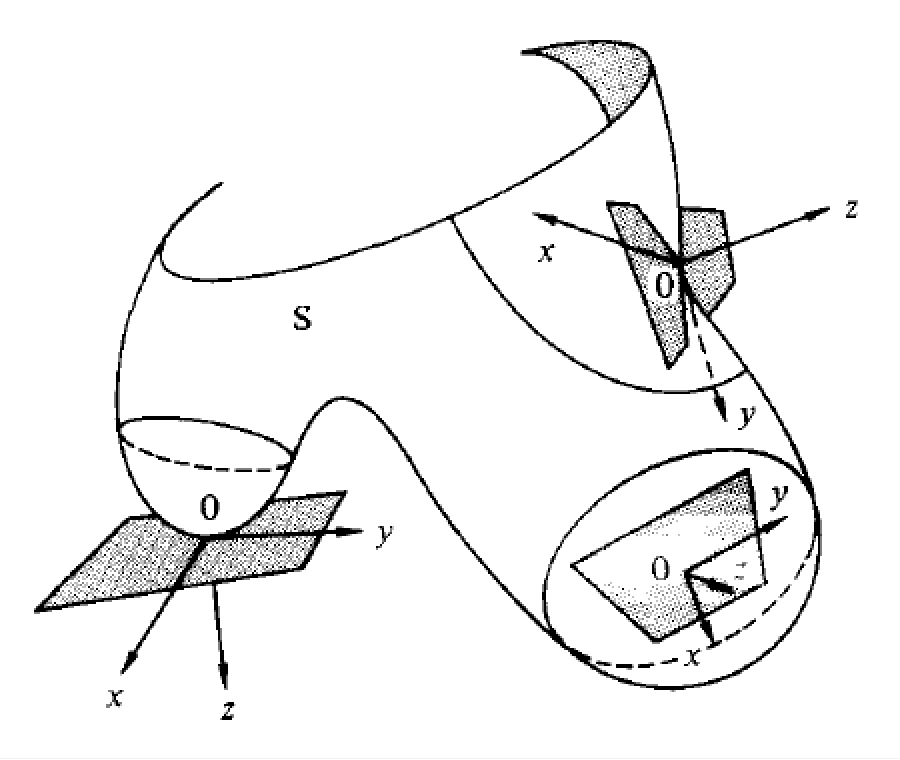
\includegraphics[scale = 0.5]{hessian_fund.png}}
\end{minipage}
\caption{\scriptsize
\textbf{Within the neighborhood of each point of the surface, we can define the function $h$ so that the surface is the graph of this function.}}
\end{figure}
\begin{solution}
We can compute the basis of the tangent space $T_{p}S$, $\mb{x}_{u}, \mb{x}_{v}$ as
\begin{align*}
\mb{x}_{u} &= (1, 0, h_{u}(u,v)); & \mb{x}_{v} &= (0, 1, h_{v}(u,v)).
\end{align*}
Thus the second-order derivatives of the parameterization are 
\begin{align*}
\mb{x}_{uu} = (0,0, h_{uu}(u,v)); && \mb{x}_{uv} = (0,0, h_{uv}(u,v)); && \mb{x}_{vv} = (0,0, h_{vv}(u,v)).
\end{align*}

Then the normal vector 
\begin{align*}
\mb{N}(u,v) &= \frac{\mb{x}_{u}\wedge \mb{x}_{v}}{\norm{\mb{x}_{u}\wedge \mb{x}_{v}}{2}}\\
&= \frac{(- h_{u}(u,v), -h_{v}(u,v), 1)}{\sqrt{1+ h^{2}_{u}(u,v) + h^{2}_{v}(u,v)}},
\end{align*}
and we can compute the coefficient for the second fundamental form as
\begin{align*}
e&= \inn{N}{\mb{x}_{uu}} \\
&= \inn{ \frac{(- h_{u}(u,v), -h_{v}(u,v), 1)}{\sqrt{1+ h^{2}_{u}(u,v) + h^{2}_{v}(u,v)}}}{ (0,0, h_{uu}(u,v)) }\\
&= \frac{h_{uu}(u,v)}{\sqrt{1+ h^{2}_{u}(u,v) + h^{2}_{v}(u,v)}};\\[10pt]
f&= \inn{N}{\mb{x}_{uv}} \\
&= \inn{ \frac{(- h_{u}(u,v), -h_{v}(u,v), 1)}{\sqrt{1+ h^{2}_{u}(u,v) + h^{2}_{v}(u,v)}}}{ (0,0, h_{uv}(u,v)) }\\
&= \frac{h_{uv}(u,v)}{\sqrt{1+ h^{2}_{u}(u,v) + h^{2}_{v}(u,v)}};\\[10pt]
g&= \inn{N}{\mb{x}_{vv}} \\
&= \inn{ \frac{(- h_{u}(u,v), -h_{v}(u,v), 1)}{\sqrt{1+ h^{2}_{u}(u,v) + h^{2}_{v}(u,v)}}}{ (0,0, h_{vv}(u,v)) }\\
&= \frac{h_{vv}(u,v)}{\sqrt{1+ h^{2}_{u}(u,v) + h^{2}_{v}(u,v)}}.
\end{align*}
So the second fundamental form at $p$ applied to vector $\mb{v}=(x,y)\in \bR^{2}$ becomes
\begin{align*}
\Pi_{\mb{x}(u,v)}((x,y))&= ex^{2} + 2f xy+ gy^{2}\\ 
&= \frac{1}{\sqrt{1+ h^{2}_{u}(u,v) + h^{2}_{v}(u,v)}} \brac{\begin{array}{cc}
x & y \end{array} }  \brac{\begin{array}{cc}
h_{uu} & h_{uv}\\ 
h_{vu} & h_{vv}
\end{array} }\brac{\begin{array}{c}
x \\ 
y
\end{array} }\\
&=\frac{1}{\sqrt{1+ h^{2}_{u}(u,v) + h^{2}_{v}(u,v)}}  \mb{v}^{T}H\mb{v},
\end{align*}
where $H$ is the Hessian matrix of $h$ w.r.t. $(u,v)$. That is, the absolute value of the quadratic term of the Taylor expansion of $f$ (via the Hessian of the function $f$) is the absolute value of the normal curvature of the graph $\cS$ of $f$.  

Also the coefficient for the first fundamental form 
\begin{align*}
E &= \inn{\mb{x}_{u}}{\mb{x}_{u}}= 1+ h^{2}_{u}; \\
F &= \inn{\mb{x}_{u}}{\mb{x}_{v}}= h_{v}h_{u}; \\
G &= \inn{\mb{x}_{v}}{\mb{x}_{v}} = 1+ h^{2}_{v}. \\
\end{align*}
Note that since $\mb{x}_{u}$ and $\mb{x}_{v}$ are not orthonormal basis for the tangent space $T_{p}S$, the matrix representation of the shape operator under $\mb{x}_{u}, \mb{x}_{v}$ is not symmetric. 

The Gaussian curvature $\mb{K} = \det\paren{dN_{p}}$ is
\begin{align*}
\mb{K} &= \frac{eg- f^{2}}{EG - F^{2}}\\
&= \frac{h_{uu}(u,v)h_{vv}(u,v)- h_{uv}^{2}(u,v)}{\paren{{1+ h^{2}_{u}(u,v) + h^{2}_{v}(u,v)}}}\frac{1}{1+h^{2}_{u}(u,v)+h^{2}_{v}(u,v) + h^{2}_{u}(u,v)h^{2}_{v}(u,v) - h_{v}^{2}(u,v)h_{u}^{2}(u,v)}\\
&= \frac{h_{uu}(u,v)h_{vv}(u,v)- h_{uv}^{2}(u,v)}{\paren{{1+ h^{2}_{u}(u,v) + h^{2}_{v}(u,v)}}}\frac{1}{1+h^{2}_{u}(u,v)+h^{2}_{v}(u,v) }\\
&=  \frac{h_{uu}(u,v)h_{vv}(u,v)- h_{uv}^{2}(u,v)}{\paren{1+ h^{2}_{u}(u,v) + h^{2}_{v}(u,v)}^{2}}
=\frac{1}{\rho^{4}}\det\paren{H},
\end{align*} where $\rho \equiv \sqrt{1+ h^{2}_{u} + h^{2}_{v}}>0.$
This shows that the shape of the surface only depends on the $\det\paren{H}= h_{uu}(u,v)h_{vv}(u,v)- h_{uv}^{2}(u,v)$.

The mean curvature $\mb{H}= \frac{-1}{2}\text{tr}\paren{dN_{p}}$ is
\begin{align*}
2\mb{H} &= \frac{eG - 2fF + gE}{EG-F^{2}}\\
&= \frac{\paren{1+ h^{2}_{v}}h_{uu} -  2h_{v}h_{u}h_{uv}+  \paren{1+ h^{2}_{u}}h_{vv}}{\paren{{1+ h^{2}_{u}(u,v) + h^{2}_{v}(u,v)}}^{3/2}}.
\end{align*}

The matrix representation of the shape operator $dN_{p}$ is given by Weingarten's equation as
\begin{align*}
-dN_{p} &=-\frac{1}{EG-F^{2}}\brac{\begin{array}{cc}
fF- eG & gF- fG \\ 
eF- fE & fF - gE
\end{array} }\\[5pt]
&= -\frac{1}{1+ h^{2}_{u}+ h^{2}_{v}}
\brac{\begin{array}{cc}
h_{v}h_{u}h_{uv}- \paren{1+ h^{2}_{v}}h_{uu}&  h_{u}h_{v}h_{vv}- h_{uv}\paren{1+ h^{2}_{v}} \\ 
h_{u}h_{v}h_{uu}- h_{uv}\paren{1+ h^{2}_{u}}  & h_{v}h_{u}h_{uv}- \paren{1+ h^{2}_{u}}h_{vv}
\end{array} }\\
&= \frac{1}{1+ h^{2}_{u}+ h^{2}_{v}}\paren{
-h_{v}h_{u}\brac{\begin{array}{cc}
h_{vu}& h_{vv} \\ 
h_{uu}& h_{uv}
\end{array} } 
+ \brac{\begin{array}{cc}
\paren{1+ h^{2}_{v}}&   0 \\ 
0 & \paren{1+ h^{2}_{u}}
\end{array} }\,
\brac{\begin{array}{cc}
h_{uu}&   h_{uv} \\ 
h_{vu} &  h_{vv}
\end{array} }
 }.
\end{align*}
This matrix is symmetric iff $F = h_{v}h_{u} = 0$. 

Note that locally any surface is the graph of a differentiable function and it shows that the second fundamental form of the surface, $-\inn{dN_{p}(\mb{v})}{\mb{v}}$, or the normal curvature of the surface at $p$ along $\mb{v}$ is given by the Hessian quadratic form, $\mb{v}^{T}H\mb{v}$ of the function. Moreover, the shape of the curve depends on the Gaussian curvature, which is proportional to the Jacobian determinant of the Hessian matrix, $\mb{K} = \det\paren{dN_{p}} \propto \det\paren{H}$. Finally, it is important to see that under basis $\set{(1,0,h_{u}), (0,1,h_{v})}$ the matrix form of $-dN_{p}\neq H$, i.e. $H$ itself is not the matrix form of the shape operator  except for the case when $h_{u}h_{v} = 0$ or $(u,v)$ is the critical point of $h$, $dh_{(u,v)} = 0$. 
\QEDA \\[20pt]
\end{solution}

\item \begin{example}
Let $h: \cS \rightarrow \bR$ be a differentiable function on surface $\cS$, and let $p\in \cS$ be a critical point of $h$, i.e. $dh_{p} = 0$. Let $\mb{w}\in T_{p}\cS$ and let $\alpha: (-\epsilon, \epsilon) \rightarrow \cS$ be a parameterized curve with $\alpha(0) = p$ and $\alpha'(0)= \mb{w}$. Let 
\begin{align*}
H_{p}h(\mb{w}) &= \rlat{\frac{d^{2} \paren{h\circ \alpha}}{dt^{2}}}{t=0}.
\end{align*}   
\begin{enumerate}
\item Let $\mb{x}: U\rightarrow \cS$ be a parameterization of $\cS$ at $p$, and show that (the fact that $p$ is a critical point here is important here)
\begin{align*}
H_{p}h(u'\mb{x}_{u}+ v'\mb{x}_{v}) &= h_{uu}(p)\paren{u'}^{2} + 2h_{uv}(p)u'v'+ h_{vv}(p)\paren{v'}^{2}.
\end{align*}
Conclude that $H_{p}h: T_{p}S \rightarrow \bR$ is a well-defined (i.e. it does not depend on the choice of $\alpha$) quadratic form on $T_{p}S$. $H_{p}h$ is also called the \emph{Hessian of $h$ at $p$}.\\[5pt]

\item Let $h: \cS \rightarrow \bR$ be the height function of $\cS$ relative to $T_{p}S$; that is, $h(q)= \inn{q-p}{N(p)}, q\in 
\cS$. Verify that $p$ is critical point of $h$ and thus that the Hessian $H_{p}h$ is well defined. Show that if $\mb{w}\in T_{p}S$, $\norm{\mb{w}}{} = 1$, then 
\begin{align*}
H_{p}h(\mb{w}) &= \text{ normal curvature at }p\text{ in the direction of }\mb{w}.
\end{align*}
Conclude that \emph{the Hessian at $p$ of the height function relative to $T_{p}S$ is the second fundamental form of $\cS$ at $p$}.
\end{enumerate}
\end{example}
\begin{solution}
\end{solution}
\end{enumerate}

\newpage
\bibliographystyle{plainnat}
\bibliography{book_reference.bib}
\end{document}